\documentclass[11pt,a4paper]{article}

\usepackage[T1]{fontenc}
\usepackage[utf8]{inputenc}
\usepackage{lmodern}
\usepackage[margin=2.4cm]{geometry}
\usepackage{amsmath,amssymb}
\usepackage{graphicx}
\usepackage{booktabs}
\usepackage{array}
\usepackage{siunitx}
\usepackage{caption}
\usepackage{subcaption}
\usepackage{float}
\usepackage[numbers,sort&compress]{natbib}
\usepackage{xcolor}
\usepackage[colorlinks=true,linkcolor=blue!50!black,citecolor=blue!50!black,urlcolor=blue!50!black]{hyperref}

\graphicspath{{../figures/}}
\sisetup{separate-uncertainty, per-mode=symbol, exponent-product=\times}
\DeclareSIUnit{\angstrom}{\text{\AA}}
\captionsetup{font=small,labelfont=bf}
\setlength{\emergencystretch}{2em}

\newcommand{\Msun}{M_\odot}
\newcommand{\Mdot}{\dot M}
\newcommand{\LEdd}{L_{\mathrm{Edd}}}
\newcommand{\rin}{r_{\mathrm{in}}}
\newcommand{\rout}{r_{\mathrm{out}}}
\newcommand{\Tmax}{T_{\max}}
\newcommand{\nupk}{\nu_{\mathrm{peak}}}
\newcommand{\rg}{r_{g}}

\title{\textbf{Thermal Emission from Geometrically Thin Accretion Disks:\\
The Role of Black Hole Mass and Accretion Rate}}
\author{\textit{[Author name(s)]}}
\date{\today}

\begin{document}
\maketitle

\begin{abstract}
\noindent
We investigate how black hole mass and accretion rate shape the thermal
continuum of a geometrically thin, optically thick accretion disk. The disk is
modelled as a set of concentric rings, each radiating as a blackbody at the
local effective temperature of the steady Newtonian thin-disk solution with a
zero-torque inner boundary at the Schwarzschild innermost stable circular
orbit, as implemented in the published \texttt{agnpy} package, with the
Planck function and physical constants taken from \texttt{astropy}. The
emission of all rings is summed numerically to obtain the
specific luminosity $L_\nu$ and the flux $F_\nu$ received by an observer at a
given distance and inclination. The numerical scheme reproduces the analytic
bolometric luminosity to a fractional accuracy of $5\times10^{-6}$ and
converges as $N^{-2}$ in the number of rings. At a fixed Eddington ratio
$L/\LEdd=0.1$, a $10\,\Msun$ black hole has a maximum disk temperature of
$\Tmax=\SI{4.4e6}{K}$ and a spectral peak at $\approx\SI{0.94}{keV}$ (soft
X-rays), while a $10^8\,\Msun$ black hole has $\Tmax=\SI{7.9e4}{K}$ and peaks
at $\approx\SI{740}{\angstrom}$ (far ultraviolet). The two peaks differ by
exactly $(10^7)^{1/4}\approx56$, reflecting the scaling
$\Tmax\propto(\Mdot/M^2)^{1/4}$. The bolometric luminosity depends only on the
accretion rate, $L=\Mdot c^2/12$, so the luminosity and the spectral peak
together determine both $\Mdot$ and $M$. We compare the model with real
observations. In SDSS quasars it matches the average far-ultraviolet
continuum slope but is too blue in the near-ultraviolet and optical, where
86--88\% of $\sim10^5$ quasars are redder than the disk predicted for their
own mass and Eddington ratio. Fitted to 48 thermal-state RXTE spectra of the
black hole binary LMC X-3, with its dynamically measured mass, it gives good
fits (median $\chi^2_\nu=0.79$) with a nearly constant spectral hardening
factor $f_{\mathrm{col}}=1.81\pm0.09$, close to the theoretical value of
$\approx1.7$. We discuss the limitations imposed by neglecting
general-relativistic effects, non-blackbody radiative transfer and additional
emission components.
\end{abstract}

\tableofcontents
\bigskip

% ===========================================================================
\section{Introduction}
% ===========================================================================

Accretion onto black holes is among the most efficient ways of converting
rest-mass energy into radiation. Black holes span more than eight orders of
magnitude in mass, from stellar-mass objects of
$\sim5$--$20\,\Msun$ in X-ray binaries to supermassive black holes of
$10^6$--$10^{10}\,\Msun$ in active galactic nuclei (AGN). Despite this range,
the same basic physics is thought to operate in both: gas with angular
momentum settles into a disk, viscous stresses transport angular momentum
outward and allow the gas to spiral inward, and the gravitational energy
released is radiated from the disk surface.

The standard model for this process is the geometrically thin, optically
thick disk of \citet{ShakuraSunyaev1973}, reviewed by \citet{Pringle1981} and
\citet{FrankKingRaine2002}. Because the disk is optically thick, each annulus
radiates approximately as a blackbody, and because the temperature falls with
radius, the total spectrum is a superposition of blackbodies with a range of
temperatures. This ``multi-colour disk'' spectrum is used to describe the
thermal component of X-ray binaries in their soft state
\citep{Mitsuda1984,RemillardMcClintock2006} and the ``big blue bump'' seen in
the optical--ultraviolet spectra of quasars \citep{Shields1978,Malkan1983}.

In this project we implement this model numerically and ask three
questions:
\begin{enumerate}
  \item How do the black hole mass $M$ and accretion rate $\Mdot$ set the
        disk temperature, the spectral peak and the total luminosity?
  \item What flux would an observer at a given distance and inclination
        measure?
  \item Why does the same physical model put the emission of stellar-mass
        black holes in the X-ray band and that of supermassive black holes
        in the ultraviolet?
  \item How well does the model describe real observations of quasars and
        of a stellar-mass black hole?
\end{enumerate}
Section~\ref{sec:theory} summarises the physical model,
Section~\ref{sec:method} describes the numerical method and its validation,
Section~\ref{sec:results} presents the results,
Section~\ref{sec:observations} compares the model with observations, and
Section~\ref{sec:discussion} connects them to observables and discusses the
limitations of the model.

% ===========================================================================
\section{Physical model}\label{sec:theory}
% ===========================================================================

\subsection{Assumptions}
We consider a steady, axisymmetric disk around a non-rotating black hole of
mass $M$ accreting at a constant rate $\Mdot$. The disk is assumed to be
\begin{itemize}
  \item \emph{geometrically thin}, $H/r\ll1$, so that it can be treated as a
        flat surface and radial pressure support is negligible;
  \item \emph{optically thick}, so that each surface element radiates as a
        blackbody at its local effective temperature;
  \item \emph{Keplerian and Newtonian}, with the inner edge at the innermost
        stable circular orbit (ISCO) of a Schwarzschild black hole,
        $\rin=6\rg$, where $\rg=GM/c^2$ is the gravitational radius.
\end{itemize}
Unless stated otherwise the outer radius is $\rout=10^5\rg$.

\subsection{Radial temperature profile}
Conservation of mass and angular momentum in a steady thin disk, together
with the assumption that the viscous torque vanishes at $\rin$, gives the
rate of energy dissipation per unit area of each face
\citep{ShakuraSunyaev1973,FrankKingRaine2002}:
\begin{equation}
  D(r)=\frac{3GM\Mdot}{8\pi r^3}\left[1-\left(\frac{\rin}{r}\right)^{1/2}\right].
\end{equation}
In local thermal equilibrium this energy is radiated as a blackbody, so
$\sigma T^4(r)=D(r)$ and
\begin{equation}
  T(r)=T_*\left(\frac{\rin}{r}\right)^{3/4}\left[1-\left(\frac{\rin}{r}\right)^{1/2}\right]^{1/4},
  \qquad
  T_*=\left(\frac{3GM\Mdot}{8\pi\sigma\rin^3}\right)^{1/4}.
  \label{eq:Tr}
\end{equation}
Far from the inner edge $T\propto r^{-3/4}$. The temperature vanishes at
$\rin$ and reaches its maximum at $r=\tfrac{49}{36}\rin$, where
\begin{equation}
  \Tmax=\left[\frac{(36/49)^3}{7}\right]^{1/4}T_*\approx0.488\,T_*.
\end{equation}
Because $\rin\propto M$, the temperature scale obeys
\begin{equation}
  \Tmax\propto\left(\frac{\Mdot}{M^2}\right)^{1/4}.
  \label{eq:Tscaling}
\end{equation}

\subsection{Luminosity and the Eddington limit}
Integrating $2D(r)$ over both faces from $\rin$ to $\rout$ gives the exact
bolometric luminosity. With $X=\rout/\rin$,
\begin{equation}
  L=\frac{3GM\Mdot}{2\rin}\left[\left(1-\frac{1}{X}\right)-\frac{2}{3}\left(1-X^{-3/2}\right)\right]
  \;\xrightarrow{X\to\infty}\;\frac{GM\Mdot}{2\rin}=\frac{\Mdot c^2}{12}.
  \label{eq:Lanalytic}
\end{equation}
The radiative efficiency of this Newtonian model is therefore $\eta=1/12$,
and the luminosity depends on $\Mdot$ alone. We parametrise the accretion
rate through the Eddington ratio $\lambda=L/\LEdd$, where
\begin{equation}
  \LEdd=\frac{4\pi GMm_pc}{\sigma_T}\approx\SI{1.26e38}{erg.s^{-1}}\left(\frac{M}{\Msun}\right)
\end{equation}
is the luminosity at which radiation pressure on electrons balances gravity
for ionised hydrogen. The accretion rate is then
$\Mdot=\lambda\LEdd/(\eta c^2)$; for a $10\,\Msun$ black hole at
$\lambda=1$ this is $\Mdot=\SI{1.68e19}{g.s^{-1}}=2.7\times10^{-7}\,\Msun\,\mathrm{yr}^{-1}$.
At fixed $\lambda$, $\Mdot\propto M$, so Eq.~\eqref{eq:Tscaling} gives
$\Tmax\propto M^{-1/4}$: \emph{more massive black holes have cooler disks}.

\subsection{Spectrum}
Each annulus of area $dA=2\pi r\,dr$ per face emits isotropically with
specific intensity $B_\nu(T)$, the Planck function \citep{RybickiLightman1979}
\begin{equation}
  B_\nu(T)=\frac{2h\nu^3}{c^2}\frac{1}{e^{h\nu/kT}-1}.
\end{equation}
The specific luminosity emitted from both faces is
\begin{equation}
  L_\nu=2\int_{\rin}^{\rout}\pi B_\nu\bigl(T(r)\bigr)\,2\pi r\,dr.
  \label{eq:Lnu}
\end{equation}
An observer at distance $D$ who views the disk at inclination $i$ (with
$i=0$ face-on) sees a projected area $dA\cos i$, so the received flux
density is
\begin{equation}
  F_\nu=\frac{\cos i}{D^2}\int_{\rin}^{\rout}B_\nu\bigl(T(r)\bigr)\,2\pi r\,dr
       =\frac{\cos i}{2\pi D^2}\,L_\nu .
  \label{eq:Fnu}
\end{equation}

The spectrum has three regimes. For $h\nu\ll kT(\rout)$ every annulus is in
the Rayleigh--Jeans limit and $L_\nu\propto\nu^2$. For $h\nu\gg k\Tmax$ the
spectrum is cut off exponentially, as in the Wien tail. In between, the
substitution $x=h\nu/kT(r)$ with $T\propto r^{-3/4}$ gives
$r\propto x^{4/3}\nu^{-4/3}$, and Eq.~\eqref{eq:Lnu} becomes
\begin{equation}
  L_\nu\propto\nu^3\int\frac{r\,dr}{e^x-1}\propto\nu^3\,\nu^{-8/3}\int\frac{x^{5/3}\,dx}{e^x-1}\propto\nu^{1/3},
\end{equation}
the characteristic signature of a multi-temperature disk.

% ===========================================================================
\section{Numerical method}\label{sec:method}
% ===========================================================================

\subsection{Model implementation and software}\label{sec:software}
Rather than re-deriving the disk model, we build on established, published
software:
\begin{itemize}
  \item \textbf{Disk model.} The temperature profile, Eq.~\eqref{eq:Tr}, is
        taken from the \texttt{SSDisk} class of \texttt{agnpy}
        \citep{Nigro2022}, an open-source, peer-reviewed Python package for
        the radiative processes of active galactic nuclei. \texttt{SSDisk}
        implements the \citet{ShakuraSunyaev1973} disk with a zero-torque
        inner boundary, following \citet{DermerMenon2009}. agnpy describes a
        disk by $(M, L_{\mathrm{disk}}, \eta, \rin, \rout)$; we pass
        $L_{\mathrm{disk}}=\eta\Mdot c^2$ with $\eta=1/12$, so agnpy's
        accretion rate equals ours exactly.
  \item \textbf{Planck function and constants.} $B_\nu(T)$ is evaluated
        with the \texttt{BlackBody} model of \texttt{astropy}
        \citep{Astropy2022}, and all physical constants come from
        \texttt{astropy.constants} (CODATA 2018 and IAU 2015 values).
\end{itemize}
What this project adds is the integration over the disk
(Section~\ref{sec:rings}). agnpy can also compute the disk spectrum itself
(\texttt{SSDisk.evaluate\_multi\_T\_bb\_sed}), using the same flux formula as
Eq.~\eqref{eq:Fnu}, but it integrates over 100 \emph{linearly} spaced radii.
That is accurate for compact disks, the case agnpy was designed for, but for
$\rout=10^5\rg$ the grid spacing is $\sim10^3\rg$ and the hot inner disk is
not resolved. We therefore use agnpy's temperature profile with our own
logarithmically spaced ring sum, and verify the two against each other in
Section~\ref{sec:validation}.

The same Shakura--Sunyaev spectrum is also standard in X-ray astronomy: it
is available in XSPEC \citep{Arnaud1996} as \texttt{ezdiskbb}
\citep{Zimmerman2005}, which uses the same zero-torque profile, and in the
simpler \texttt{diskbb} \citep{Mitsuda1984}, which uses a pure
$T\propto r^{-3/4}$ law.

\subsection{Ring discretisation}\label{sec:rings}
The code (\texttt{accretion\_disk/disk.py}) works in CGS units throughout.
The disk is divided into $N$ rings whose
edges $r_0=\rin<r_1<\dots<r_N=\rout$ are logarithmically spaced, so every
decade in radius receives equal resolution. Ring $k$ is assigned the
temperature $T_k=T(\bar r_k)$ at its geometric-mean radius
$\bar r_k=\sqrt{r_kr_{k+1}}$ and the one-face area
$A_k=\pi(r_{k+1}^2-r_k^2)$. Equations~\eqref{eq:Lnu} and~\eqref{eq:Fnu}
become sums over rings,
\begin{equation}
  L_\nu=2\pi\sum_{k=0}^{N-1}B_\nu(T_k)\,A_k,\qquad
  F_\nu=\frac{\cos i}{D^2}\sum_{k=0}^{N-1}B_\nu(T_k)\,A_k ,
  \label{eq:ringsum}
\end{equation}
which are evaluated for all frequencies at once as a matrix--vector product.
The default is $N=2000$. The Planck function is set to exactly zero for
$h\nu/kT>600$, where it is below $10^{-255}$ of its peak, to avoid
floating-point overflow in the Wien tail.

Figure~\ref{fig:rings} illustrates the method: grouping the 2000 rings into
eight zones shows that each zone contributes a nearly blackbody spectrum,
while their sum is the broad multi-temperature disk spectrum.

\begin{figure}[H]
  \centering
  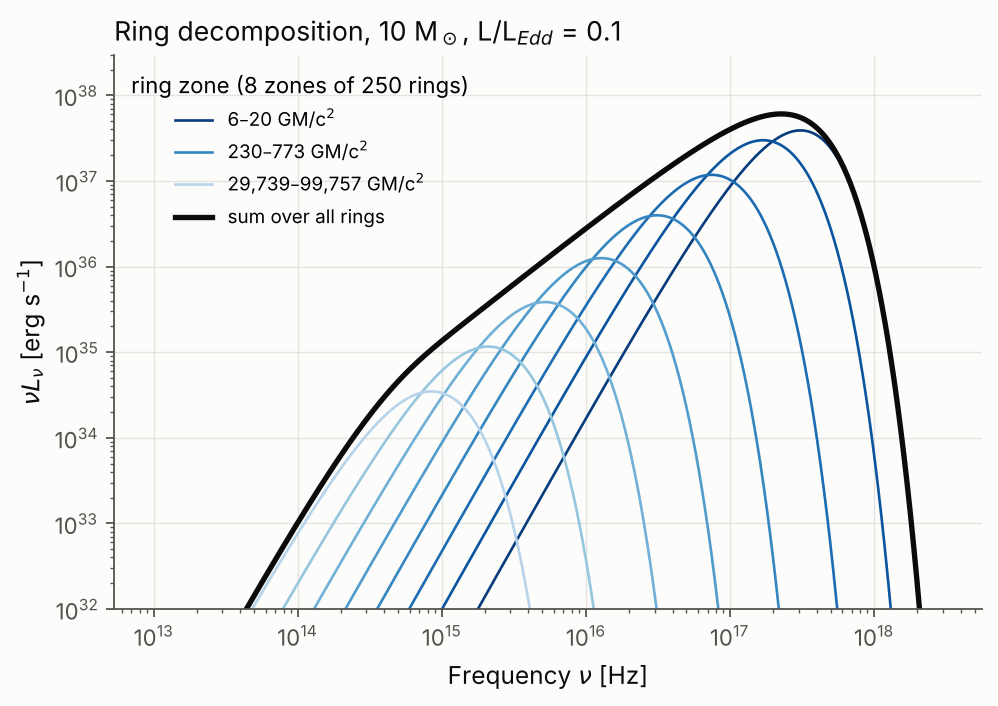
\includegraphics[width=0.75\textwidth]{fig8_ring_decomposition.png}
  \caption{Decomposition of the disk spectrum of a $10\,\Msun$ black hole at
  $\lambda=0.1$. Coloured curves show the summed emission of eight zones of
  250 rings each, from the hot inner zone (dark) to the cool outer zone
  (light); the black curve is the total. Each zone is close to a blackbody,
  but the total is much broader.}
  \label{fig:rings}
\end{figure}

\subsection{Derived quantities}
The bolometric luminosity is computed directly from the rings as
$L=2\sigma\sum_kT_k^4A_k$. The peak frequency $\nupk$ of $\nu L_\nu$ is found
on a logarithmic grid of 4000 frequencies spanning $10^{-5}$ to $40$ times
$k\Tmax/h$; the grid maximum is refined by fitting a parabola to the three
neighbouring points in $\log\nu$--$\log(\nu L_\nu)$ space. Scaling the grid
with $\Tmax$ gives the same relative resolution for every mass and
accretion rate.

\subsection{Validation}\label{sec:validation}
The implementation is checked by an automated test suite
(\texttt{tests/test\_disk.py}, 22 tests). Table~\ref{tab:validation}
summarises the main checks against analytic results and against agnpy.

\begin{table}[H]
  \centering
  \caption{Validation of the numerical model against analytic results and
  against agnpy.}
  \label{tab:validation}
  \begin{tabular}{@{}ll@{}}
    \toprule
    Check & Result \\
    \midrule
    $\pi\int B_\nu\,d\nu=\sigma T^4$ & agrees to $<10^{-4}$ \\
    Ring sum of $\sigma T^4$ vs.\ Eq.~\eqref{eq:Lanalytic} & $5.4\times10^{-6}$ ($N=2000$) \\
    $\int L_\nu\,d\nu$ vs.\ Eq.~\eqref{eq:Lanalytic} & $9.5\times10^{-6}$ \\
    Location and value of $\Tmax$ & $r=\tfrac{49}{36}\rin$, $\Tmax=0.488\,T_*$ \\
    Low-frequency slope & $L_\nu\propto\nu^{2.00}$ \\
    Intermediate slope ($\rout=10^8\rg$) & $L_\nu\propto\nu^{0.33}$ \\
    Mass scaling at fixed $\lambda$ & $\nupk\propto M^{-0.2500}$ \\
    Accretion-rate scaling at fixed $M$ & $\nupk\propto\Mdot^{0.2500}$, $L\propto\Mdot^{1.000}$ \\
    Observer geometry & $F_\nu\propto\cos i/D^2$, face-on $F_\nu=L_\nu/2\pi D^2$ \\
    $T(r)$ vs.\ closed form, Eq.~\eqref{eq:Tr} & identical to $<10^{-10}$ \\
    $\nu F_\nu$ vs.\ agnpy SED ($\rout=50\rg$) & agrees to $<\SI{0.3}{\percent}$ \\
    \bottomrule
  \end{tabular}
\end{table}

Figure~\ref{fig:convergence} shows the convergence of the ring sum. The
error in the bolometric luminosity falls as $N^{-2}$, as expected for a
midpoint-type rule; about 100 rings give \SI{0.2}{\percent} accuracy, and
the default of 2000 rings gives errors well below $10^{-5}$, negligible
compared with the physical uncertainties of the model.

\begin{figure}[H]
  \centering
  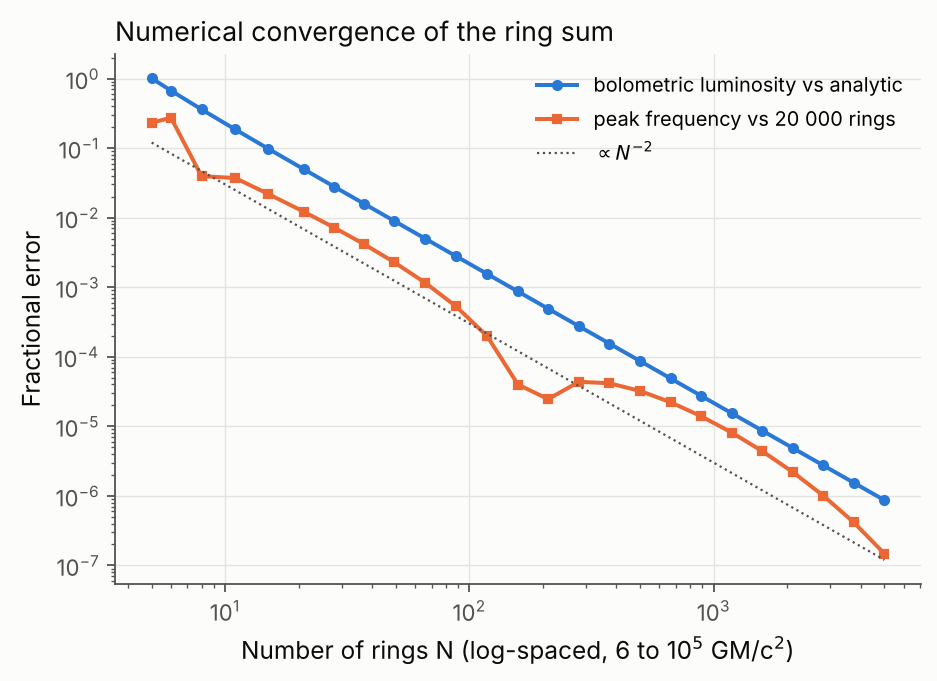
\includegraphics[width=0.62\textwidth]{fig7_convergence.png}
  \caption{Fractional error of the bolometric luminosity (relative to
  Eq.~\ref{eq:Lanalytic}) and of the peak frequency (relative to a
  20\,000-ring calculation) as a function of the number of rings $N$.}
  \label{fig:convergence}
\end{figure}

Figure~\ref{fig:agnpy} compares our ring sum with agnpy's own spectrum
calculation. For compact disks ($\rout\le50\rg$), where agnpy's 100-point
linear grid is adequate, the two agree to \SI{0.1}{\percent} at all
frequencies that carry significant flux. This confirms that our code
computes the same Shakura--Sunyaev spectrum as the published package. As
$\rout$ grows, agnpy's grid becomes too coarse to resolve the inner disk: at
$\rout=10^3\rg$ it underestimates the flux at $h\nu=10\,k\Tmax$ by a factor
of five, and at $\rout=10^5\rg$ it misses the spectral peak entirely.

\begin{figure}[H]
  \centering
  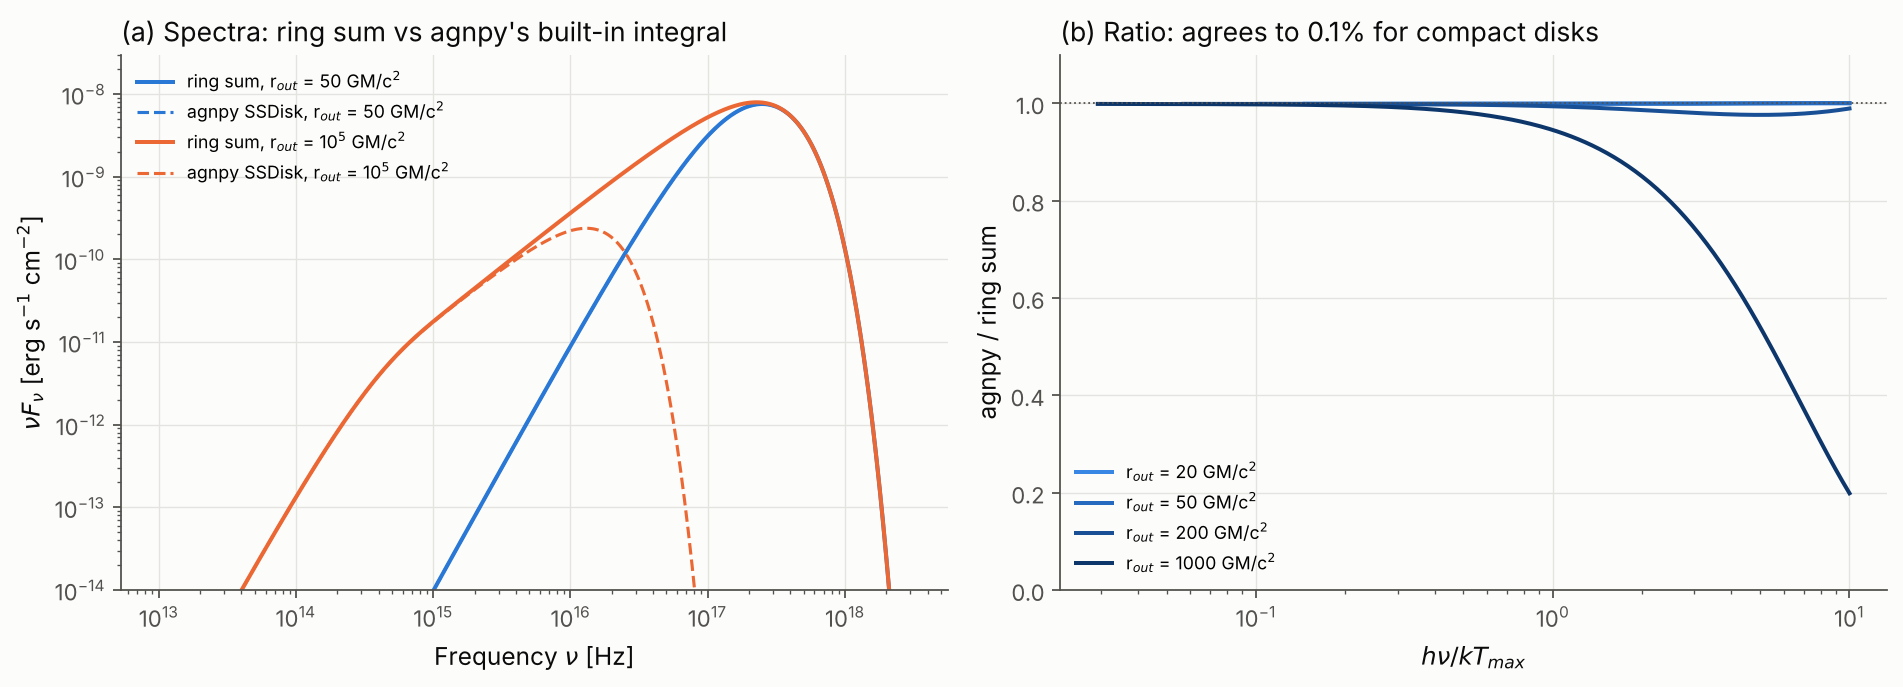
\includegraphics[width=\textwidth]{fig9_agnpy_crosscheck.png}
  \caption{(a) $\nu F_\nu$ of a $10\,\Msun$ disk at $\lambda=0.1$
  (\SI{8}{kpc}, $i=\ang{60}$) from our ring sum (solid) and from agnpy's
  built-in integration (dashed), for $\rout=50\rg$ (the curves overlap) and
  $\rout=10^5\rg$. (b) Ratio of agnpy's result to the ring sum for several
  disk sizes.}
  \label{fig:agnpy}
\end{figure}

% ===========================================================================
\section{Results}\label{sec:results}
% ===========================================================================

We adopt two representative systems, both accreting at $\lambda=0.1$:
\begin{itemize}
  \item a \textbf{stellar-mass black hole} of $10\,\Msun$ at
        $D=\SI{8}{kpc}$ viewed at $i=\ang{60}$, typical of a Galactic X-ray
        binary;
  \item a \textbf{supermassive black hole} of $10^8\,\Msun$ at
        $D=\SI{100}{Mpc}$ viewed at $i=\ang{30}$, typical of a Seyfert
        nucleus or quasar.
\end{itemize}
Their properties at three Eddington ratios are listed in
Table~\ref{tab:summary}.

\begin{table}[H]
  \centering
  \caption{Disk properties of the representative systems. $\nupk$ and
  $E_{\mathrm{peak}}=h\nupk$ refer to the peak of $\nu L_\nu$;
  $F_{\mathrm{bol}}$ is the bolometric flux at the stated distance and
  inclination ($D=\SI{8}{kpc}$, $i=\ang{60}$ for $10\,\Msun$;
  $D=\SI{100}{Mpc}$, $i=\ang{30}$ for $10^8\,\Msun$).}
  \label{tab:summary}
  \small
  \begin{tabular}{@{}lccccccc@{}}
    \toprule
    $M$ & $L/\LEdd$ & $\Mdot$ & $L_{\mathrm{bol}}$ & $\Tmax$ & $\nupk$ & $E_{\mathrm{peak}}$ & $F_{\mathrm{bol}}$ \\
    $[\Msun]$ & & [$\Msun\,\mathrm{yr}^{-1}$] & [erg\,s$^{-1}$] & [K] & [Hz] & [keV] & [erg\,s$^{-1}$\,cm$^{-2}$] \\
    \midrule
    10 & 0.01 & \num{2.7e-9} & \num{1.26e37} & \num{2.49e6} & \num{1.28e17} & 0.53 & \num{1.6e-9} \\
    10 & 0.1  & \num{2.7e-8} & \num{1.26e38} & \num{4.42e6} & \num{2.27e17} & 0.94 & \num{1.6e-8} \\
    10 & 1    & \num{2.7e-7} & \num{1.26e39} & \num{7.86e6} & \num{4.04e17} & 1.67 & \num{1.6e-7} \\
    \midrule
    $10^8$ & 0.01 & \num{2.7e-2} & \num{1.26e44} & \num{4.42e4} & \num{2.27e15} & 0.0094 & \num{1.8e-10} \\
    $10^8$ & 0.1  & \num{2.7e-1} & \num{1.26e45} & \num{7.86e4} & \num{4.04e15} & 0.0167 & \num{1.8e-9} \\
    $10^8$ & 1    & \num{2.7}    & \num{1.26e46} & \num{1.40e5} & \num{7.18e15} & 0.0297 & \num{1.8e-8} \\
    \bottomrule
  \end{tabular}
\end{table}

\subsection{Temperature structure}
Figure~\ref{fig:Tprofile} shows the temperature profiles of the two systems.
Expressed in units of $\rg$, the profiles have identical shapes: a steep rise
from zero at the ISCO, a maximum at $8.2\,\rg$, and a $T\propto r^{-3/4}$
decline. Only the normalisation differs. The inner disk of the
$10\,\Msun$ black hole reaches $\SI{4.4e6}{K}$, while that of the
$10^8\,\Msun$ black hole reaches only $\SI{7.9e4}{K}$, even though it
radiates $10^7$ times more power. The ratio of the two temperatures is
exactly $(10^7)^{1/4}=56.2$, as required by Eq.~\eqref{eq:Tscaling}. The
supermassive disk can be cooler because its emitting area, $\propto M^2$,
is $10^{14}$ times larger. The zero-torque boundary condition lowers the
temperature at the maximum by a factor of $7^{1/4}\approx1.6$ relative to
the pure power law (dotted lines), and drives it to zero at $\rin$.

\begin{figure}[H]
  \centering
  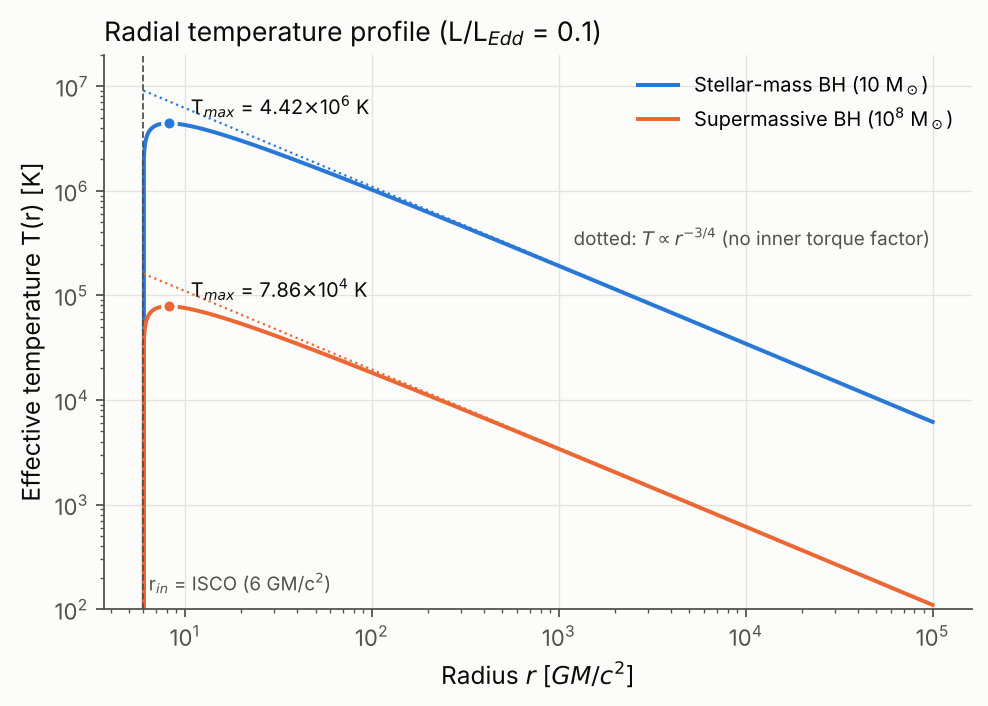
\includegraphics[width=0.72\textwidth]{fig1_temperature_profiles.png}
  \caption{Effective temperature as a function of radius for a $10\,\Msun$
  and a $10^8\,\Msun$ black hole at $\lambda=0.1$. Dots mark $\Tmax$ at
  $r=\tfrac{49}{36}\rin$; dotted lines show the $T\propto r^{-3/4}$ power law
  without the inner-boundary factor.}
  \label{fig:Tprofile}
\end{figure}

\subsection{Stellar-mass versus supermassive black holes}
Figure~\ref{fig:compare} compares the spectra. The $10\,\Msun$ disk peaks at
$\nupk=\SI{2.27e17}{Hz}$ ($E\approx\SI{0.94}{keV}$), in the soft X-ray band,
which matches the thermal disk component observed in black hole X-ray
binaries in their high/soft state \citep{RemillardMcClintock2006}. The
$10^8\,\Msun$ disk peaks at $\nupk=\SI{4.04e15}{Hz}$
($\lambda\approx\SI{740}{\angstrom}$), in the far ultraviolet, consistent with
the big blue bump in quasar spectra \citep{Shields1978,Malkan1983}.

The spectral \emph{shape} is the same in both cases when frequency is
expressed in units of $k\Tmax/h$: we find $h\nupk=2.466\,k\Tmax$ for the peak
of $\nu L_\nu$ and $h\nu=0.80\,k\Tmax$ for the peak of $L_\nu$, independent
of $M$ and $\Mdot$. The single model therefore produces characteristic
frequencies that differ by a factor of 56 simply because $\Tmax\propto
M^{-1/4}$ at fixed Eddington ratio. Both spectra show the three regimes of
Section~\ref{sec:theory}: a Rayleigh--Jeans $\nu^2$ tail below the
temperature of the outer edge ($T(\rout)\approx\SI{6200}{K}$ for the stellar
disk and $\approx\SI{110}{K}$ for the supermassive disk), a $\nu^{1/3}$
section ($\nu L_\nu\propto\nu^{4/3}$) at intermediate frequencies, and a Wien
cutoff above $\nupk$.

\begin{figure}[H]
  \centering
  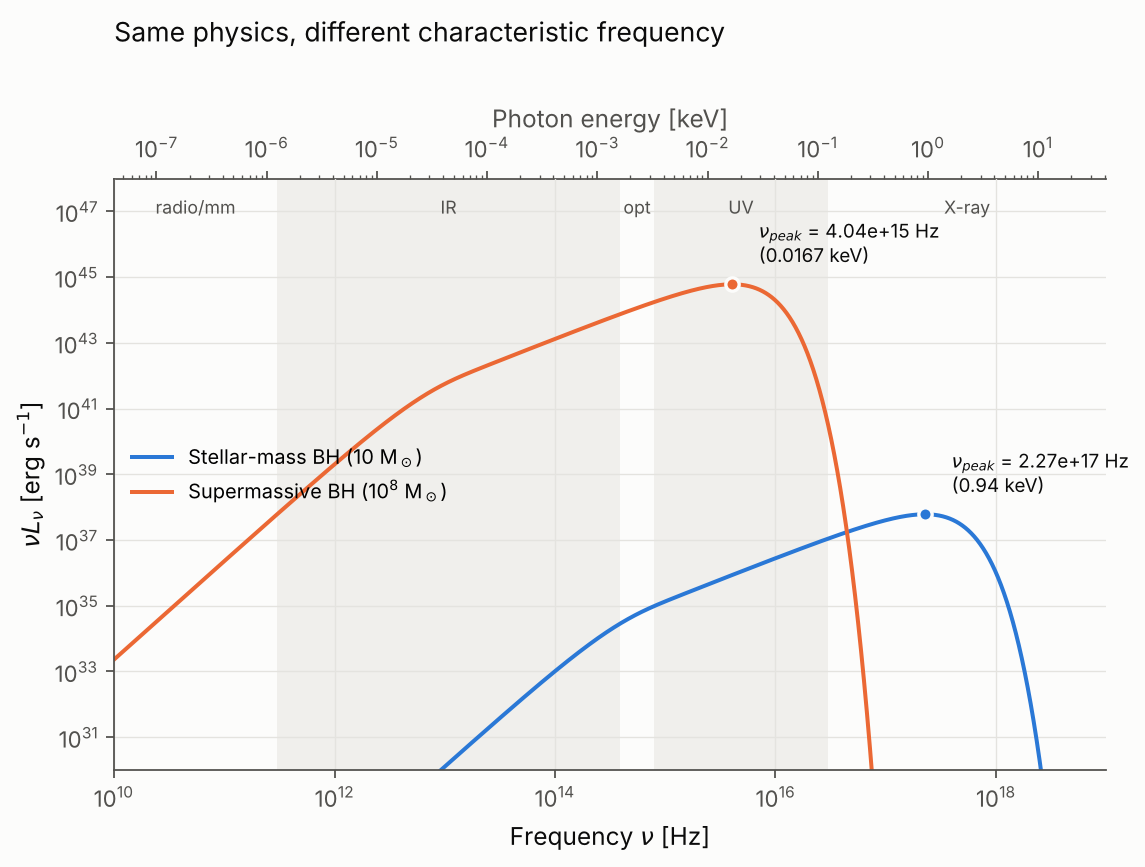
\includegraphics[width=0.8\textwidth]{fig2_spectra_stellar_vs_smbh.png}
  \caption{Spectral energy distributions $\nu L_\nu$ of the $10\,\Msun$ and
  $10^8\,\Msun$ disks at $\lambda=0.1$. Shaded bands mark the IR and UV
  regions; the top axis gives the photon energy.}
  \label{fig:compare}
\end{figure}

\subsection{Dependence on black hole mass}
Figure~\ref{fig:mass} shows a sequence of masses from $10$ to $10^9\,\Msun$ at
fixed $\lambda=0.1$. Increasing the mass raises the luminosity in proportion
($L\propto\Mdot\propto M$) and moves the peak to lower frequency, so the
peaks lie along the locus $\nu L_\nu\propto\nupk^{-4}$ (dashed line). A
power-law fit to the peak frequencies gives a slope of $-0.2500$, in exact
agreement with $\nupk\propto M^{-1/4}$. Over this mass range the peak moves
from the X-ray band, through the extreme ultraviolet, into the far
ultraviolet.

\begin{figure}[H]
  \centering
  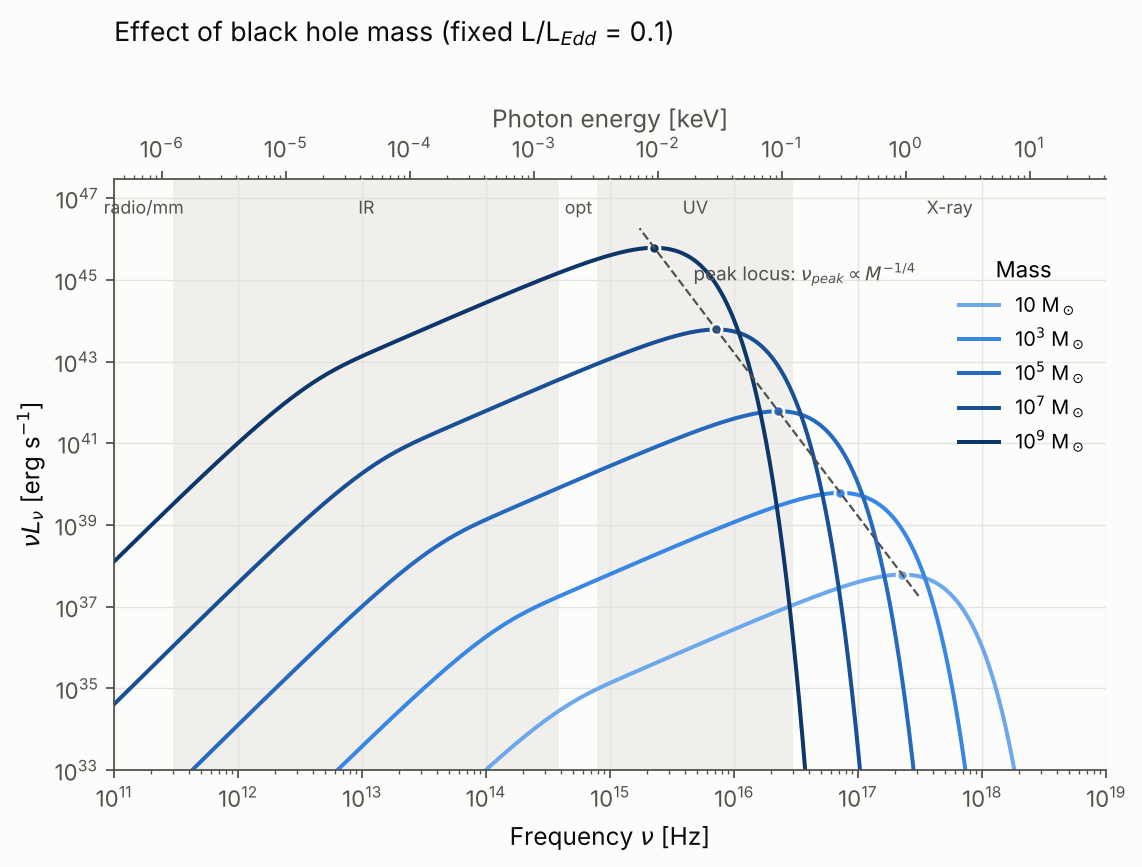
\includegraphics[width=0.8\textwidth]{fig3_vary_mass.png}
  \caption{Disk spectra for black hole masses of $10$, $10^3$, $10^5$, $10^7$
  and $10^9\,\Msun$ at $\lambda=0.1$. Dots mark the peak of each spectrum;
  the dashed line traces the peak locus.}
  \label{fig:mass}
\end{figure}

\subsection{Dependence on accretion rate}
Figure~\ref{fig:mdot} shows the effect of varying the accretion rate from
$\lambda=0.01$ to $1$ at fixed mass. The luminosity increases in proportion
to $\Mdot$, but the peak moves only as $\Mdot^{1/4}$: a hundredfold increase
in accretion rate shifts $\nupk$ by a factor of only $100^{1/4}\approx3.2$
(from 0.53 to \SI{1.67}{keV} for the stellar-mass disk). In the
$\nu^{1/3}$ regime the spectra at different $\Mdot$ are parallel, with
$L_\nu\propto\Mdot^{2/3}$ at fixed frequency.

\begin{figure}[H]
  \centering
  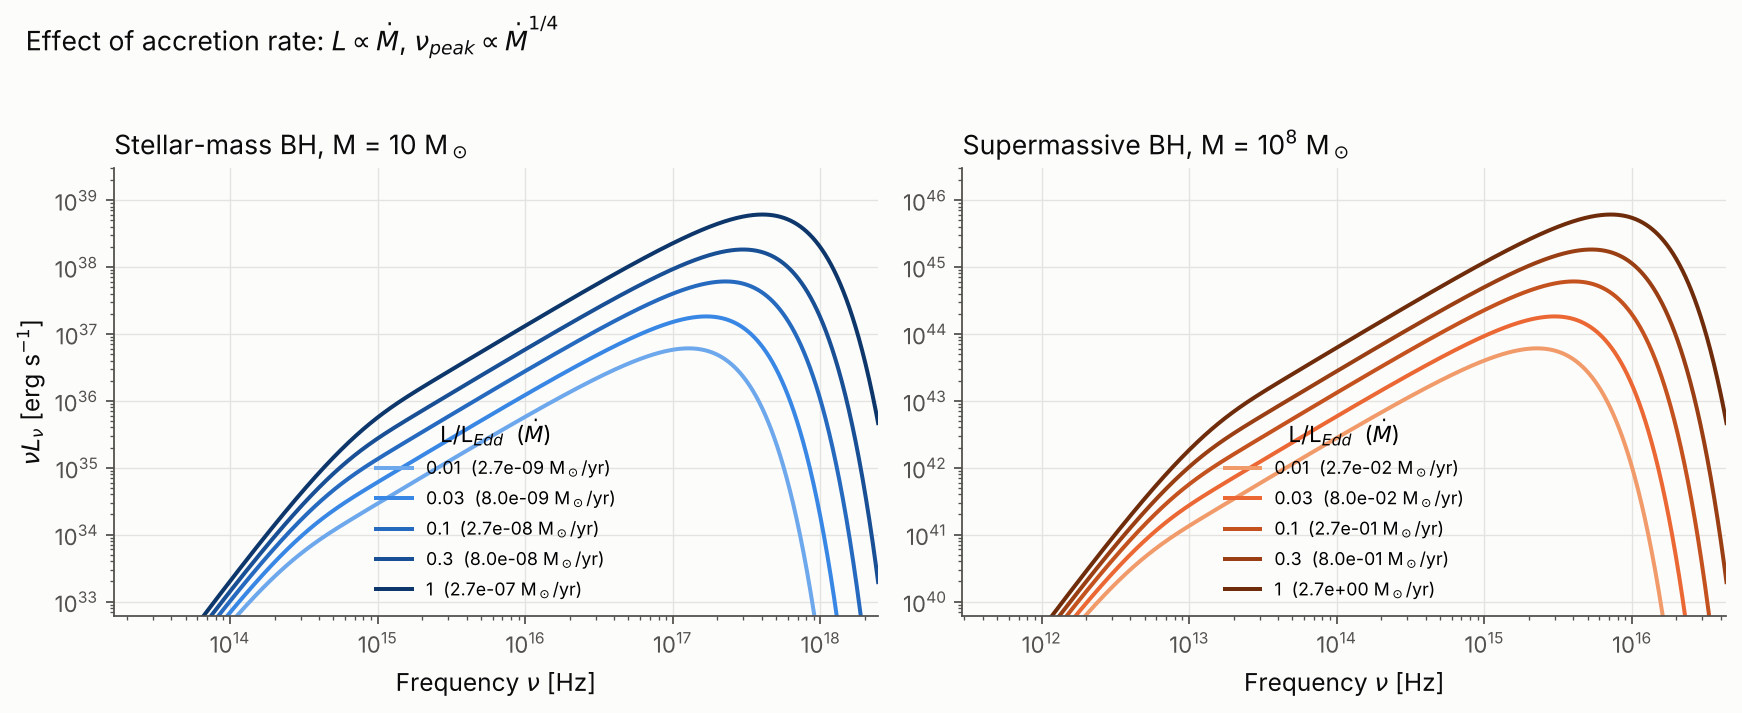
\includegraphics[width=\textwidth]{fig4_vary_accretion_rate.png}
  \caption{Disk spectra for Eddington ratios $\lambda=0.01$--$1$ for the
  $10\,\Msun$ (left) and $10^8\,\Msun$ (right) black holes. The legend gives
  the corresponding accretion rate.}
  \label{fig:mdot}
\end{figure}

\subsection{Scaling relations}
Figure~\ref{fig:scalings} summarises the scaling laws. At fixed Eddington
ratio $\nupk\propto M^{-1/4}$ (panel a); at fixed mass
$\nupk\propto\Mdot^{1/4}$ (panel b); and the bolometric luminosity lies on
the single relation $L=\Mdot c^2/12$ for every mass (panel c). Combining
these, the model results can be written compactly as
\begin{align}
  \Tmax &\approx \SI{4.4e6}{K}\left(\frac{M}{10\,\Msun}\right)^{-1/4}\left(\frac{\lambda}{0.1}\right)^{1/4},\\
  \nupk &\approx \SI{2.3e17}{Hz}\left(\frac{M}{10\,\Msun}\right)^{-1/4}\left(\frac{\lambda}{0.1}\right)^{1/4}.
\end{align}

\begin{figure}[H]
  \centering
  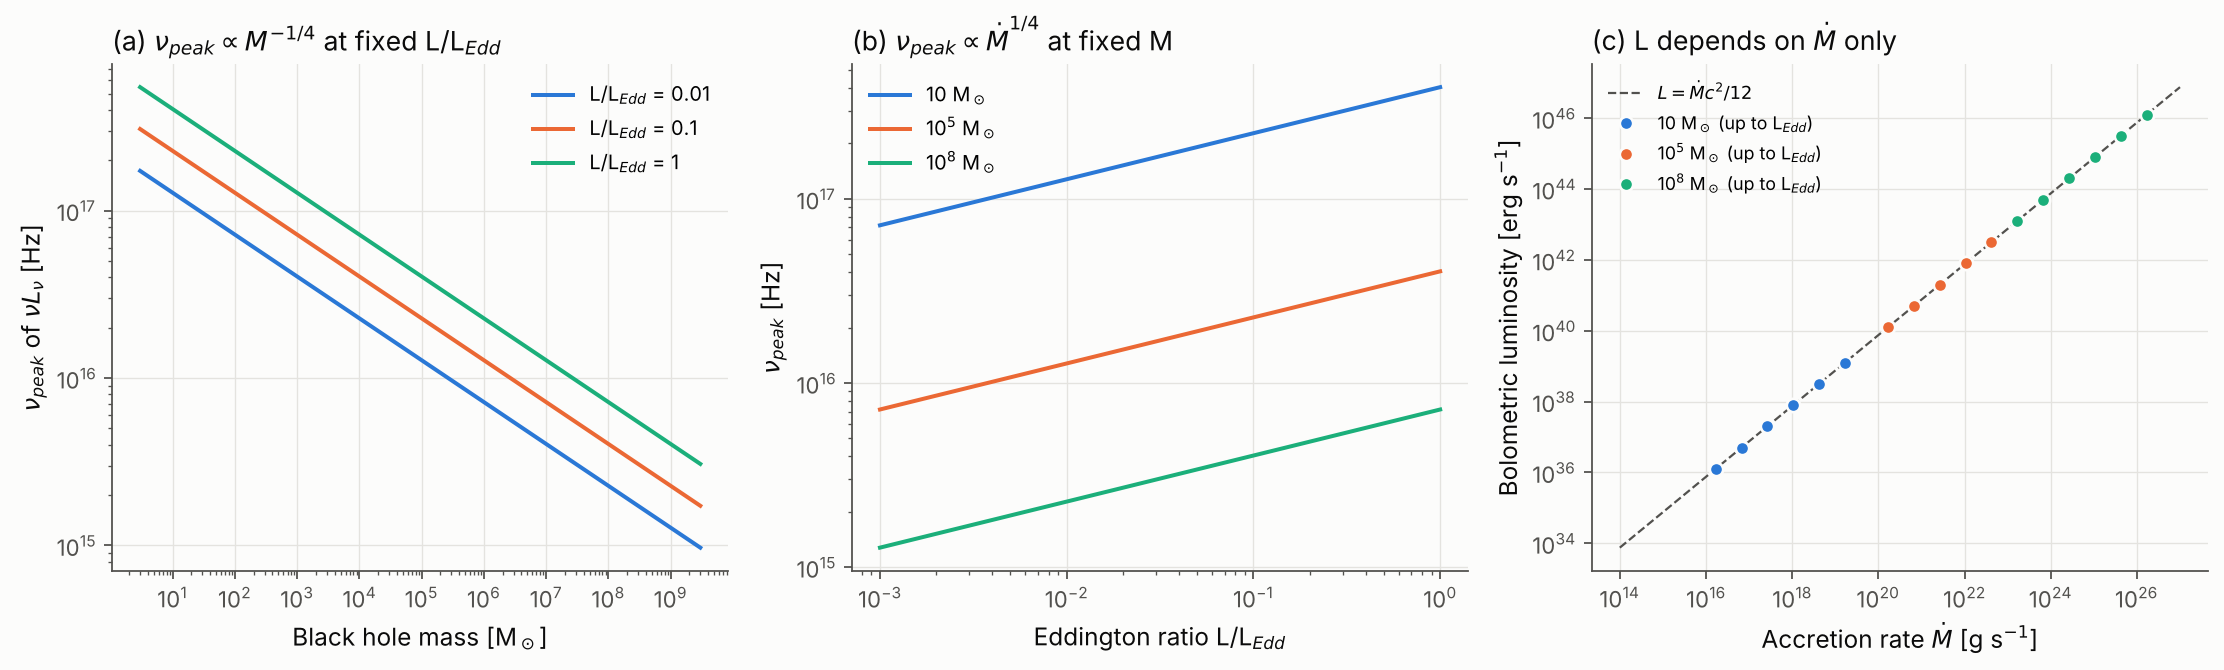
\includegraphics[width=\textwidth]{fig5_scaling_relations.png}
  \caption{(a) Peak frequency versus black hole mass at three Eddington
  ratios. (b) Peak frequency versus Eddington ratio at three masses.
  (c) Bolometric luminosity versus accretion rate; points for all masses
  lie on $L=\Mdot c^2/12$.}
  \label{fig:scalings}
\end{figure}

\subsection{Observed flux: distance and inclination}
Figure~\ref{fig:flux} shows the flux received by observers of the two
fiducial systems at several inclinations. At $\lambda=0.1$ the X-ray binary
at \SI{8}{kpc} and $i=\ang{60}$ has a bolometric flux of
$\SI{1.6e-8}{erg.s^{-1}.cm^{-2}}$, typical of a bright Galactic X-ray
source. The AGN at \SI{100}{Mpc} and $i=\ang{30}$ has
$\SI{1.8e-9}{erg.s^{-1}.cm^{-2}}$, its far greater luminosity being largely
offset by its $1.25\times10^4$ times greater distance.

In this non-relativistic model inclination affects only the normalisation
through $\cos i$; the spectral shape is unchanged. Going from face-on to
$i=\ang{85}$ reduces the flux by a factor of 11. An observer who assumes
isotropic emission and infers $L_{\mathrm{iso}}=4\pi D^2F$ obtains
$L_{\mathrm{iso}}=2\cos i\,L$, which overestimates the true luminosity by up
to a factor of two for face-on disks ($L_{\mathrm{iso}}/L=1.73$ for the AGN
at $i=\ang{30}$) and underestimates it for $i>\ang{60}$.

\begin{figure}[H]
  \centering
  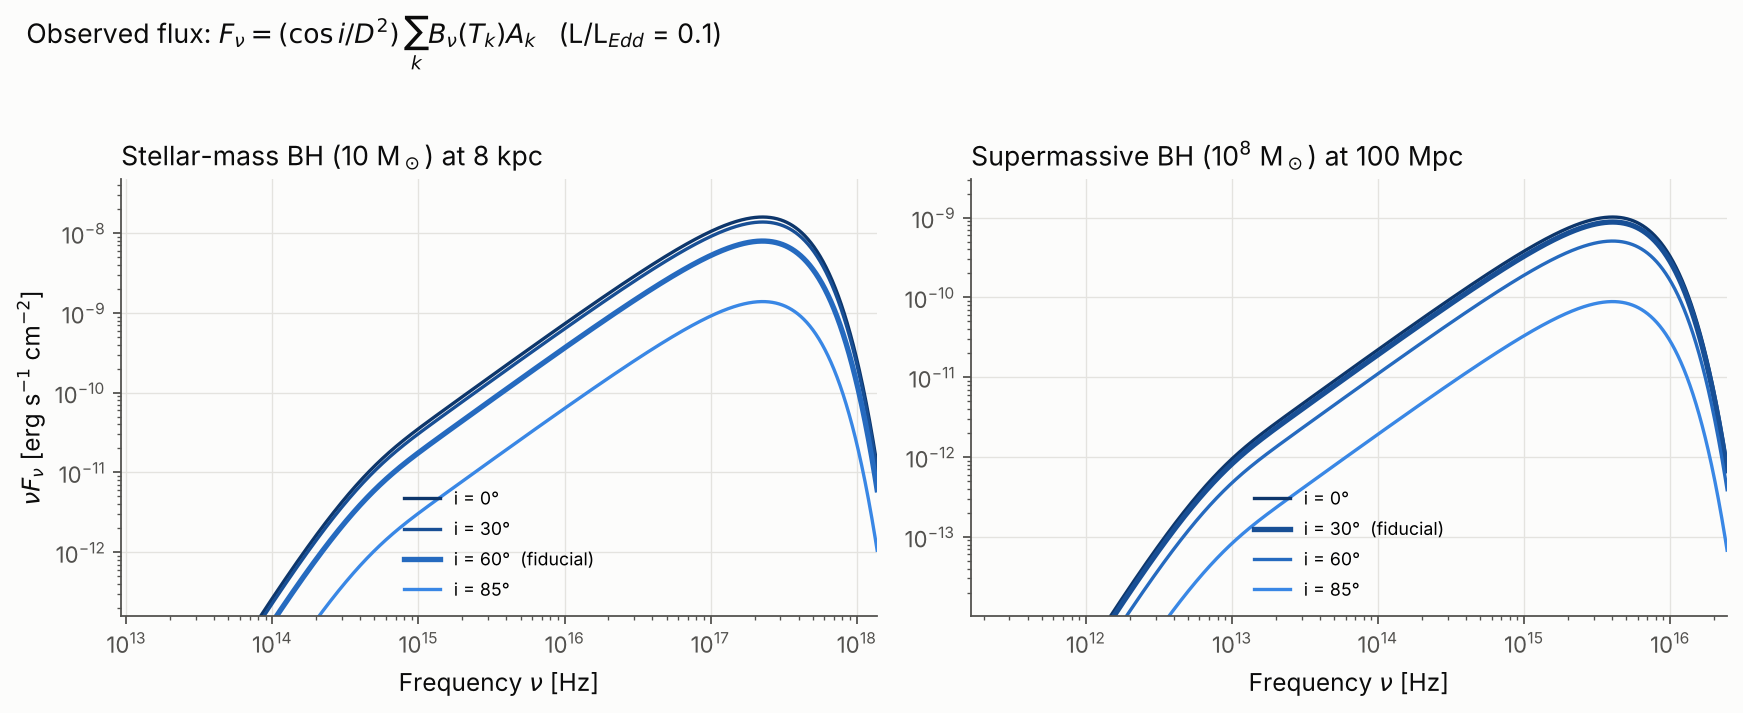
\includegraphics[width=\textwidth]{fig6_observed_flux.png}
  \caption{Observed $\nu F_\nu$ for the $10\,\Msun$ black hole at
  \SI{8}{kpc} (left) and the $10^8\,\Msun$ black hole at \SI{100}{Mpc}
  (right), both at $\lambda=0.1$, for inclinations of
  \ang{0}, \ang{30}, \ang{60} and \ang{85}. The fiducial inclination is
  drawn with a thicker line.}
  \label{fig:flux}
\end{figure}

% ===========================================================================
\section{Comparison with observations}\label{sec:observations}
% ===========================================================================

We now test the model against three real datasets
(Table~\ref{tab:obsdata}). Two concern supermassive black holes, through the
optical--ultraviolet continua of quasars; the third is a stellar-mass black
hole, through X-ray spectra. All data were downloaded from public archives
with \texttt{fetch\_observations.py} and analysed with
\texttt{compare\_observations.py}, both in the \texttt{scripts/} directory.

\begin{table}[H]
  \centering
  \caption{Observational data used in this section.}
  \label{tab:obsdata}
  \small
  \begin{tabular}{@{}>{\raggedright\arraybackslash}p{3.8cm}>{\raggedright\arraybackslash}p{5.0cm}>{\raggedright\arraybackslash}p{6.4cm}@{}}
    \toprule
    Dataset & Content & Compared with \\
    \midrule
    SDSS composite quasar \citep{VandenBerk2001} & median spectrum of 2204 quasars, 800--8555\,\AA &
      disk spectrum of a typical SDSS quasar \\
    SDSS DR7 quasar catalogue \citep{Shen2011} & virial $M$, $L/\LEdd$ and continuum slopes of $\sim10^5$ quasars &
      model slope for each quasar's own $M$ and $L/\LEdd$ \\
    RXTE/PCA spectra of LMC X-3 (HEASARC) & 65 pointings, 1996--1999, 3--20\,keV &
      model folded through the detector response, with $M$, $i$, $D$ from \citet{Orosz2014} \\
    \bottomrule
  \end{tabular}
\end{table}

\subsection{The SDSS composite quasar spectrum}
\citet{VandenBerk2001} combined 2204 SDSS quasar spectra into a median
composite. Measured through their continuum windows at 1350--1365 and
4200--4230\,\AA, the composite has $f_\nu\propto\nu^{\alpha_\nu}$ with
$\alpha_\nu=-0.47$. The paper quotes $-0.44$ for 1300--5000\,\AA.
Figure~\ref{fig:obscomposite} compares the composite with the disk spectrum
of a typical SDSS DR7 quasar, taken as the sample medians
$M=10^{9.0}\,\Msun$ and $L/\LEdd=0.17$ (so $\Tmax=\SI{5.1e4}{K}$), normalised
at 1350\,\AA.

For such a disk the spectral peak lies near 1100\,\AA, so the 1350--4200\,\AA\
range is on the rising side of the peak rather than in the $\nu^{1/3}$
regime, and the model gives $\alpha_\nu=-0.24$. The disk shape is
qualitatively right: it has the turnover in the far UV that defines the
``big blue bump''. However, it is bluer than the composite, and it falls well
below the composite longward of $\sim4000$\,\AA. There the composite
steepens to $\alpha_\nu=-2.45$, which \citet{VandenBerk2001} attribute partly
to host-galaxy starlight, a component the disk model does not include.

\begin{figure}[H]
  \centering
  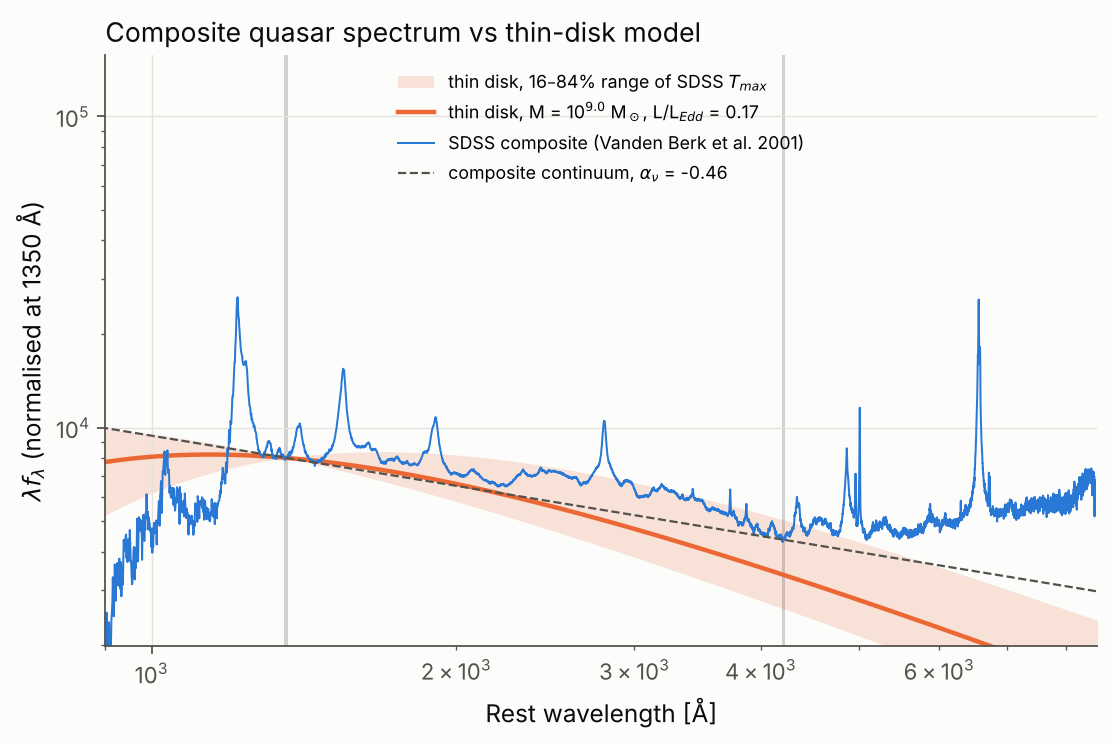
\includegraphics[width=0.8\textwidth]{obs1_composite_quasar.png}
  \caption{SDSS median composite quasar spectrum \citep{VandenBerk2001}
  (blue) compared with the thin-disk model for the median mass and
  Eddington ratio of SDSS DR7 quasars (orange line). The shaded band spans
  the 16--84\% range of $\Tmax$ in that sample. All curves are normalised in
  the 1350--1365\,\AA\ window. Grey bars mark the two continuum windows; the
  dashed line is the composite's power-law continuum.}
  \label{fig:obscomposite}
\end{figure}

\subsection{Continuum slopes of individual SDSS quasars}
A more direct test uses individual quasars. For every SDSS DR7 quasar,
\citet{Shen2011} list a virial black hole mass and an Eddington ratio. They
also list the slope $\alpha_\lambda$ of a local power-law continuum
$f_\lambda\propto\lambda^{\alpha_\lambda}$, fitted together with an iron
template in fixed rest-frame windows around C\,\textsc{iv}
([1445,1465]+[1700,1705]\,\AA), Mg\,\textsc{ii}
([2200,2700]+[2900,3090]\,\AA) and H$\beta$ ([4435,4700]+[5100,5535]\,\AA).
Their Eddington ratios use bolometric corrections from the mean quasar SED
of \citet{Richards2006}.

For each quasar we compute the slope that the disk model predicts in the
same windows, given that quasar's $M$ and $L/\LEdd$. For fixed $\rout/\rg$
the disk spectrum has a universal shape set by $\Tmax$ alone, with
$\Tmax\propto(\lambda_{\mathrm{Edd}}/M)^{1/4}$. The model slope can
therefore be tabulated once as a function of $\Tmax$ and interpolated for
each object. We use non-BAL quasars with slope uncertainty $<0.3$ and median
S/N$\ge5$ in the line region.

\begin{table}[H]
  \centering
  \caption{Observed continuum slopes of SDSS DR7 quasars \citep{Shen2011}
  compared with the thin-disk prediction for each quasar's own mass and
  Eddington ratio. Ranges are 16th--84th percentiles; ``obs$-$model'' is
  the median difference and ``redder'' the fraction of quasars with a larger
  (redder) $\alpha_\lambda$ than predicted.}
  \label{tab:slopes}
  \small
  \begin{tabular}{@{}lrcccc@{}}
    \toprule
    Window & $N$ & observed $\alpha_\lambda$ & model $\alpha_\lambda$ &
      obs$-$model & redder \\
    \midrule
    C\,\textsc{iv} & 19\,020 & $-1.30$ ($-1.74$, $-0.78$) & $-1.32$ ($-1.70$, $-0.78$) & $-0.03$ & 48\% \\
    Mg\,\textsc{ii} & 65\,594 & $-1.36$ ($-1.71$, $-0.98$) & $-1.86$ ($-2.03$, $-1.60$) & $+0.46$ & 86\% \\
    H$\beta$ & 16\,472 & $-1.51$ ($-2.03$, $-0.82$) & $-2.14$ ($-2.22$, $-2.00$) & $+0.61$ & 88\% \\
    \bottomrule
  \end{tabular}
\end{table}

The results (Table~\ref{tab:slopes}, Figure~\ref{fig:obsslopes}) are mixed.
In the far UV (C\,\textsc{iv}), the observed and predicted distributions
agree in both median and width. In the near UV and optical, real quasars
are systematically redder than the disk, by $\Delta\alpha_\lambda\approx0.5$
(Mg\,\textsc{ii}) and $0.6$ (H$\beta$). The predicted H$\beta$ slopes lie
close to the $\nu^{1/3}$ limit, $\alpha_\lambda=-7/3$, but the observed ones
are much shallower and more widely spread.

The lower panels of Figure~\ref{fig:obsslopes} show a second difference. The
model predicts that the slope should flatten steeply for cooler disks, but
the observed median slope barely changes with the $\Tmax$ inferred from
$M$ and $L/\LEdd$. The far-UV agreement in the median is therefore partly a
coincidence of where the model curve crosses the data.

Several effects not in the model plausibly contribute:
\begin{itemize}
  \item dust reddening in the host galaxy;
  \item host-galaxy starlight in the H$\beta$ windows;
  \item Balmer-continuum and Fe\,\textsc{ii} emission near Mg\,\textsc{ii};
  \item the $\sim0.4$\,dex uncertainty of single-epoch virial masses, which
        blurs any trend with $\Tmax$.
\end{itemize}
The model may also be incomplete for AGN disks: its outer regions are
self-gravitating, and their atmospheres are not blackbodies.

\begin{figure}[H]
  \centering
  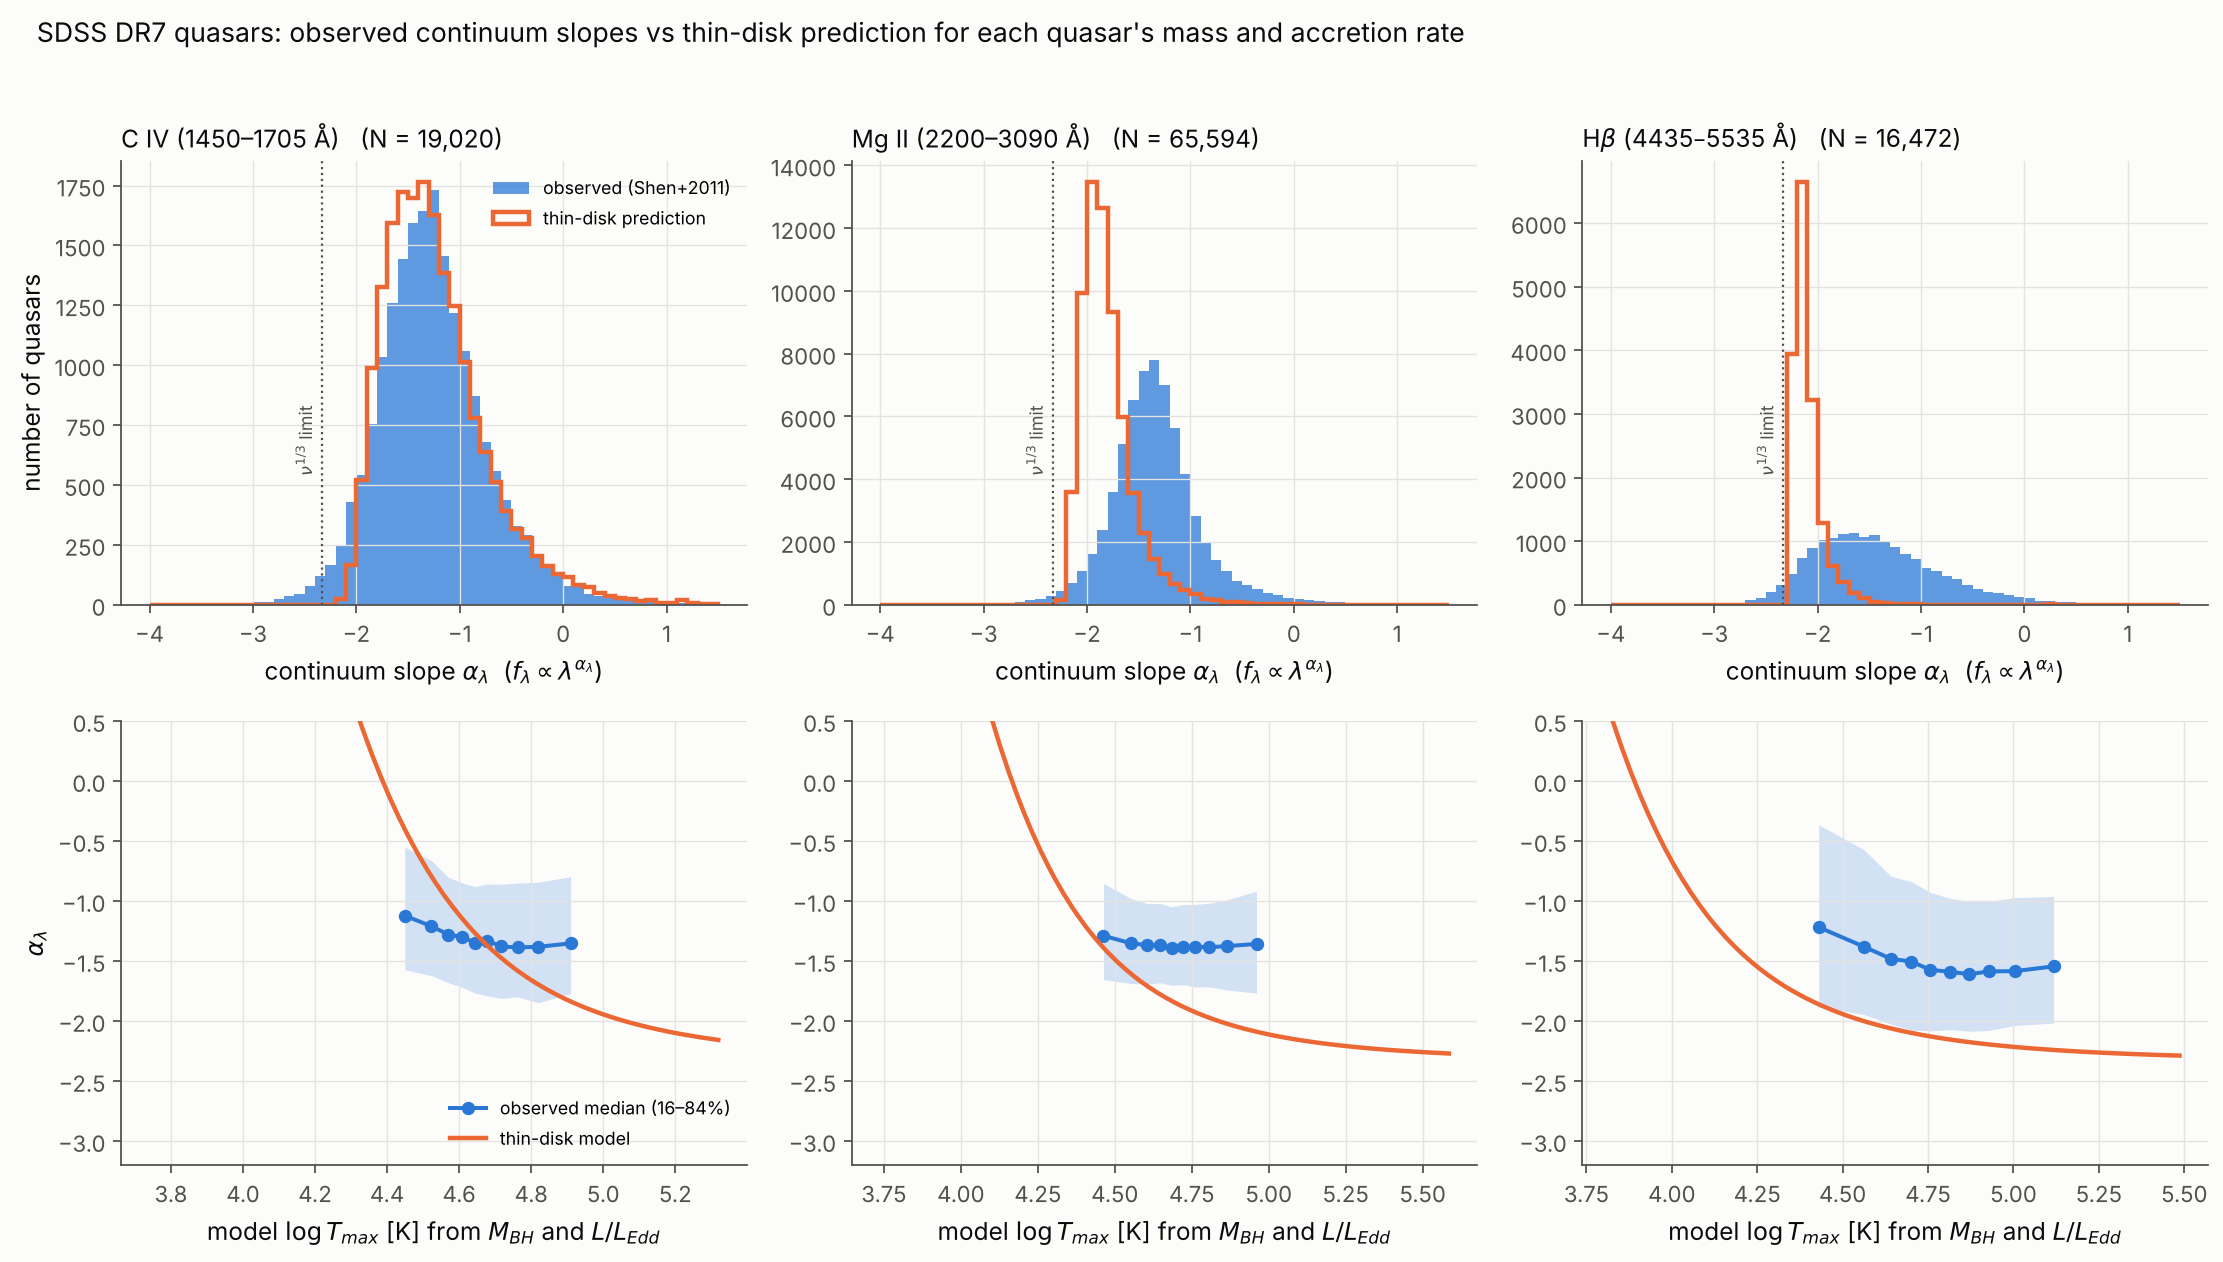
\includegraphics[width=\textwidth]{obs2_quasar_slopes.png}
  \caption{Top: distributions of the observed continuum slope $\alpha_\lambda$
  \citep{Shen2011} (filled) and of the thin-disk prediction for the same
  quasars (outline) in the C\,\textsc{iv}, Mg\,\textsc{ii} and H$\beta$
  windows. The dotted line marks the $\nu^{1/3}$ limit,
  $\alpha_\lambda=-7/3$. Bottom: observed median slope (points; shading
  16--84\%) in bins of the model $\Tmax$ inferred from each quasar's mass and
  Eddington ratio, compared with the model prediction (line).}
  \label{fig:obsslopes}
\end{figure}

\subsection{X-ray spectra of the black hole binary LMC X-3}
LMC X-3 is a persistent black hole X-ray binary in the Large Magellanic
Cloud. It is usually in a disk-dominated (thermal) state and has little
interstellar absorption, which makes it a clean test of thin-disk models.
Its black hole mass $M=6.98\pm0.56\,\Msun$ and inclination
$i=69.24\pm0.72^\circ$ were measured dynamically by \citet{Orosz2014}. We
adopt the LMC distance $D=48.1\pm2.2$\,kpc used for LMC~X-1 by
\citet{Orosz2009}, as \citet{Steiner2014} did.

\paragraph{Data.} We use the RXTE Proportional Counter Array (PCA)
standard-product spectra from the HEASARC archive: all 65 pointings of
1996--1999 with at least 3\,ks of exposure. Each pointing comes with a
source spectrum, a background spectrum and a response matrix, summed over
the PCA detectors (effective area $\approx\SI{6400}{cm^2}$ at 8\,keV).

We fit the background-subtracted count rates over 3--20\,keV, adding a 1\%
systematic error per channel as \citet{Steiner2014} did. The absorbing column
$N_{\mathrm H}=4\times10^{20}$\,cm$^{-2}$ attenuates the flux by less than
1\% above 3\,keV, so we neglect it.

\paragraph{Model.} The ring-sum disk of Section~\ref{sec:method} is used with
$M$, $i$ and $D$ fixed to the values above. Each ring radiates a
colour-corrected (diluted) blackbody, $f_{\mathrm{col}}^{-4}B_\nu(f_{\mathrm{col}}T)$.
The hardening factor $f_{\mathrm{col}}$ raises the colour temperature without
changing the emitted flux \citep{ShimuraTakahara1995}. A power law
represents the weak Comptonised tail.

The model photon spectrum is folded through each response matrix and
fitted by least squares. There are four free parameters: $\Mdot$,
$f_{\mathrm{col}}$, and the power-law normalisation and index. With $\rin$
fixed at $6\rg$, these determine both the colour temperature and the
normalisation, $\propto\cos i\,\rin^2/(D^2f_{\mathrm{col}}^4)$, so
$f_{\mathrm{col}}$ is constrained by the data. Following \citet{Steiner2014},
we call a spectrum thermal-state if the disk provides more than 75\% of the
3--20\,keV counts and $\chi^2_\nu<2$. 48 of the 65 spectra qualify.

\begin{figure}[H]
  \centering
  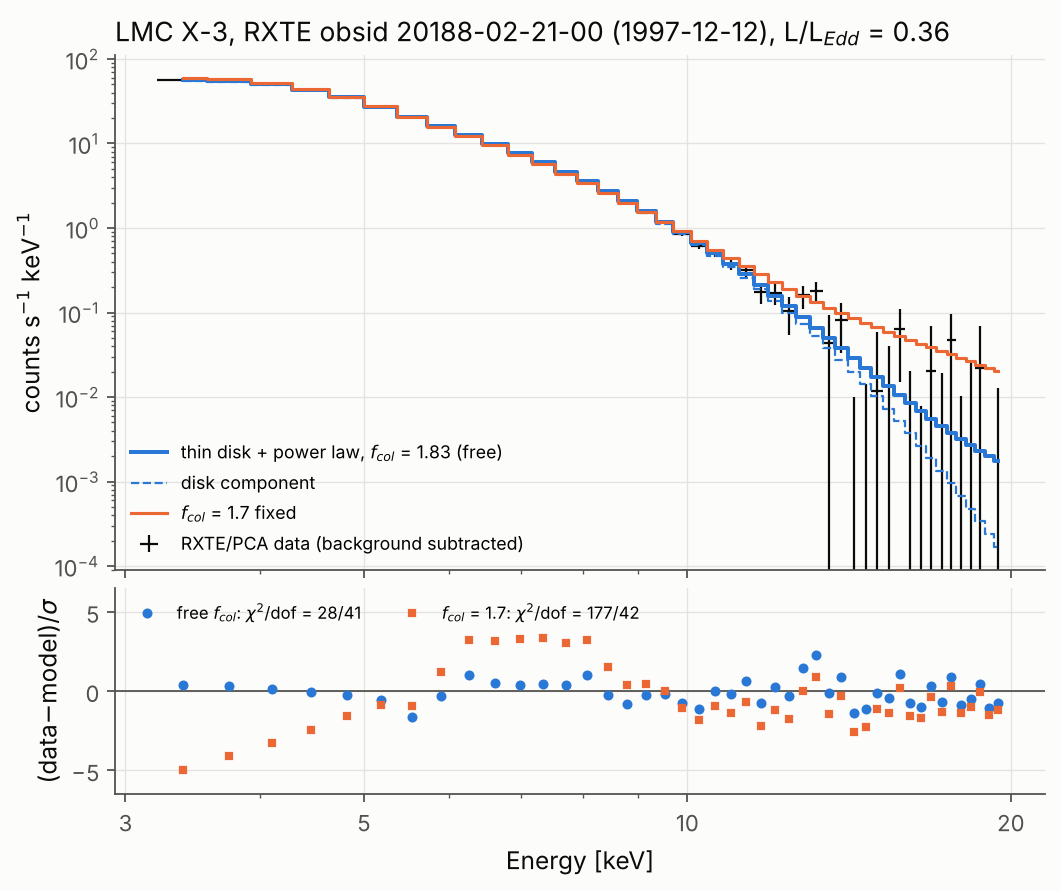
\includegraphics[width=0.72\textwidth]{obs3_lmcx3_spectrum.png}
  \caption{RXTE/PCA spectrum of LMC X-3 (obsid 20188-02-21-00, 1997
  December 12) with the best-fitting thin disk plus power law
  ($f_{\mathrm{col}}$ free, blue) and with $f_{\mathrm{col}}=1.7$ fixed
  (orange). The lower panel shows the residuals.}
  \label{fig:obsspec}
\end{figure}

\paragraph{Results.} Figure~\ref{fig:obsspec} shows a representative fit.
With $f_{\mathrm{col}}$ free, the model describes the thermal-state spectra
well, with median $\chi^2_\nu=0.79$. The fitted Eddington ratios span
$L/\LEdd\approx0.16$--$0.87$; these are model-dependent, as discussed below.
The required hardening factor is remarkably stable from spectrum to spectrum
(Figure~\ref{fig:obspop}a):
\begin{equation}
  f_{\mathrm{col}}=1.81\ \ (\text{16--84\%: }1.78\text{--}1.83)\ \pm0.09\ (\text{syst.}).
\end{equation}
The systematic error is obtained by refitting all thermal-state spectra
with $M$, $D$ and $i$ each shifted by $\pm1\sigma$
(Table~\ref{tab:fcolsyst}); the mass dominates. This value agrees with the
theoretical $f_{\mathrm{col}}\approx1.7$ of \citet{ShimuraTakahara1995}.

Fixing $f_{\mathrm{col}}=1.7$ raises the median $\chi^2_\nu$ to 3.3, mainly
because the model's temperature and normalisation cannot then be adjusted
independently. Pure blackbody rings ($f_{\mathrm{col}}=1$) are strongly
excluded (median $\chi^2_\nu=117$), which directly demonstrates the
spectral hardening discussed in Section~\ref{sec:discussion}.

The bolometric disk flux scales as $F\propto T_{\mathrm{col}}^{4.4}$
(Figure~\ref{fig:obspop}b), close to the $F\propto T^4$ expected if the inner
disk edge stays at a fixed radius. This reproduces the result, found with
relativistic models, that the inner disk of LMC X-3 sits at a stable
radius, identified with the ISCO \citep{Steiner2014}.

\begin{table}[H]
  \centering
  \caption{Median fitted $f_{\mathrm{col}}$ of the 48 thermal-state spectra
  when the adopted system parameters are varied by $\pm1\sigma$.}
  \label{tab:fcolsyst}
  \small
  \begin{tabular}{@{}lccc@{}}
    \toprule
    Parameter & $-1\sigma$ & fiducial & $+1\sigma$ \\
    \midrule
    $M$ ($6.98\pm0.56\,\Msun$) & 1.732 & 1.806 & 1.877 \\
    $D$ ($48.1\pm2.2$\,kpc) & 1.848 & 1.806 & 1.766 \\
    $i$ ($69.24\pm0.72^\circ$) & 1.820 & 1.806 & 1.790 \\
    \bottomrule
  \end{tabular}
\end{table}

\begin{figure}[H]
  \centering
  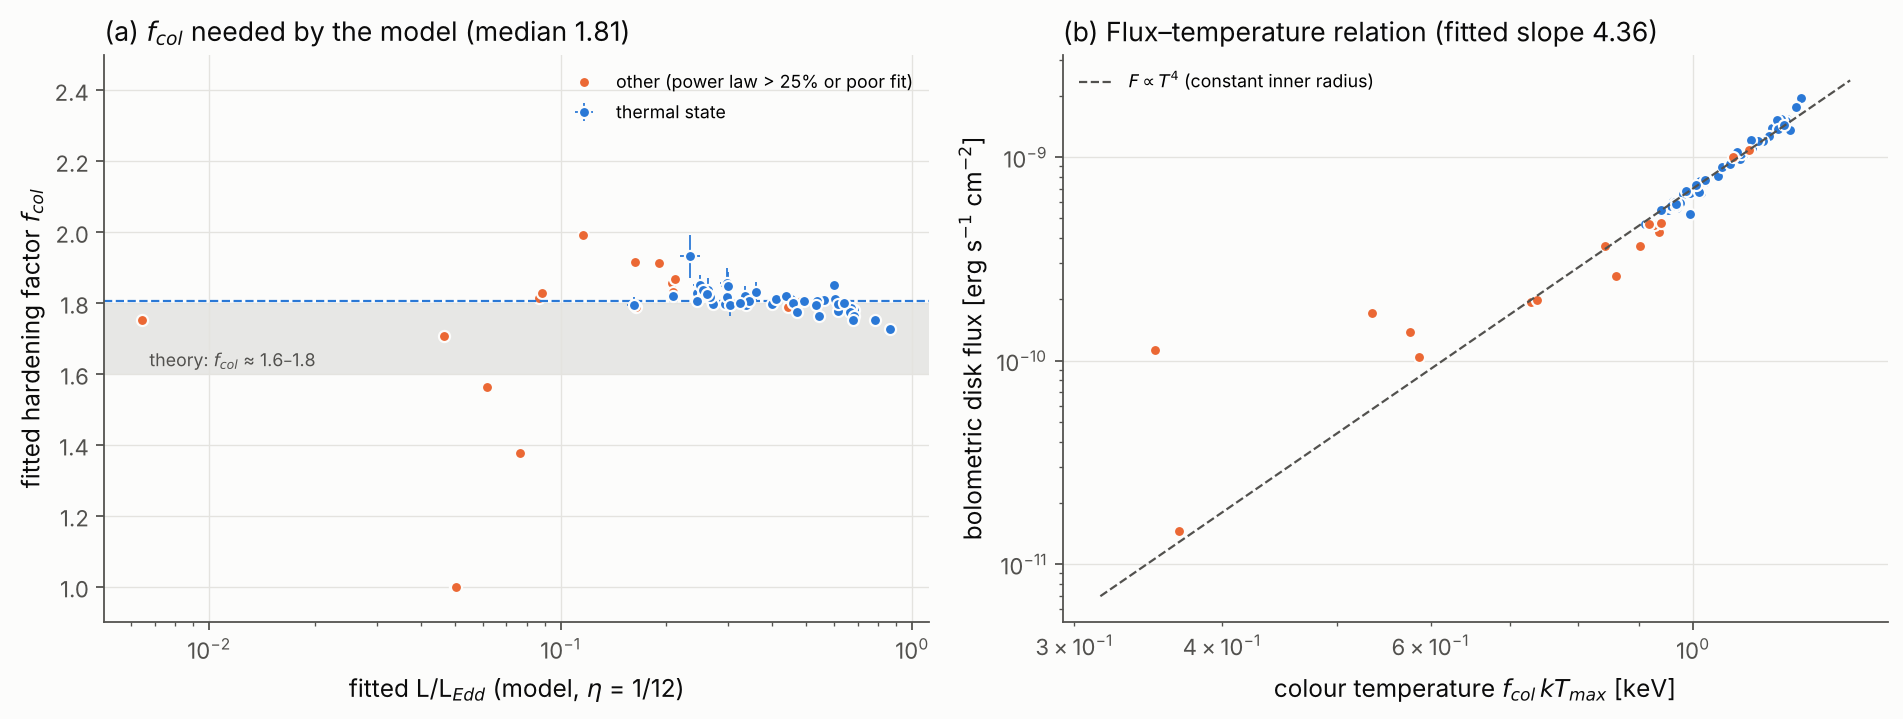
\includegraphics[width=\textwidth]{obs4_lmcx3_population.png}
  \caption{Fits to 65 RXTE/PCA spectra of LMC X-3. (a) Fitted hardening
  factor versus fitted Eddington ratio. Blue: thermal-state spectra (with
  $1\sigma$ errors); orange: other spectra. The dashed line is the
  thermal-state median, and the grey band the theoretical range. (b)
  Bolometric disk flux versus colour temperature $f_{\mathrm{col}}k\Tmax$,
  with the $F\propto T^4$ relation for a constant inner radius.}
  \label{fig:obspop}
\end{figure}

\paragraph{Caveats.} The fitted luminosities depend on the Newtonian
efficiency ($\eta=1/12$) and on the neglect of relativistic effects, which
are important at $i\approx\ang{69}$. They should be taken as indicative.
For comparison, \citet{Steiner2014}, using the fully relativistic
\textsc{kerrbb2} model, found that only 391 of their 1454 thermal-state
spectra lay in the range $L/\LEdd=0.05$--0.3, so LMC X-3 is frequently more
luminous than that. Our $f_{\mathrm{col}}$ likewise absorbs any shortcomings
of the Newtonian model, as well as the PCA flux calibration (the Crab-based
correction of \citet{Steiner2014} would change it by $\sim$2--3\%). It is
therefore an effective hardening factor rather than a pure measurement of
disk-atmosphere physics.

\subsection{What the comparisons show}
The stellar-mass case is a success. With an independently measured mass,
the model reproduces the X-ray spectra of LMC X-3 over a range of
luminosities with a single, physically sensible hardening factor. The
quasar case is only a partial success. The disk explains the existence and
far-UV location of the big blue bump, but real quasar continua are redder
in the near-UV and optical than a bare thin disk. Explaining that difference
requires components and effects outside the model
(Section~\ref{sec:discussion}).

% ===========================================================================
\section{Discussion}\label{sec:discussion}
% ===========================================================================

\subsection{Connecting observables to accretion physics}
The results show how the two basic parameters of the accretion flow map onto
observable spectral properties.
\begin{itemize}
  \item \textbf{The bolometric luminosity measures the accretion rate.}
        Because $L=\eta\Mdot c^2$ with a mass-independent efficiency, a
        luminosity measurement (from the flux, distance and inclination)
        gives $\Mdot$ directly, but carries no information about $M$.
  \item \textbf{The spectral peak measures the temperature scale.} The peak
        frequency gives $\Tmax\propto(\Mdot/M^2)^{1/4}$, a combination of
        mass and accretion rate.
  \item \textbf{Together they determine the mass.} Eliminating $\Mdot$
        between $L=\Mdot c^2/12$ and Eq.~\eqref{eq:Tr} gives
        \begin{equation}
          M=\left[\frac{3G\Mdot}{8\pi\sigma T_*^4\,(6G/c^2)^3}\right]^{1/2}
          \propto L^{1/2}\,\Tmax^{-2}.
        \end{equation}
        Applying this inversion to synthetic spectra recovers the input mass
        to \SI{0.03}{\percent} for both the stellar-mass and supermassive
        cases (see the accompanying notebook). This is the principle behind
        continuum-fitting estimates of black hole mass and, with relativistic
        models, spin.
\end{itemize}
The weak, fourth-root dependence of temperature on both parameters explains
why disks around black holes of similar type have similar characteristic
energies: stellar-mass disks cluster around \SIrange{0.5}{2}{keV}, and AGN
disks peak in the ultraviolet. It also means that a large change in
accretion rate produces only a modest shift in the spectral peak but a large
change in luminosity.

\subsection{Limitations}
The model captures the essential physics of thermal disk emission, but
several effects that matter in comparisons with real data are neglected.

\paragraph{General-relativistic disk structure.} The Newtonian temperature
profile should be replaced by the relativistic solution of
\citet{NovikovThorne1973}. More importantly, black hole spin moves the ISCO
from $6\rg$ (non-rotating) to as close as $1\rg$ for a maximally rotating
black hole with a prograde disk \citep{Bardeen1972}. This increases the
radiative efficiency from $\approx\SI{5.7}{\percent}$ (Schwarzschild, compared
with our Newtonian $1/12\approx\SI{8.3}{\percent}$) to as much as
$\approx\SI{42}{\percent}$, makes the inner disk hotter, and shifts $\nupk$
upward. Our results therefore correspond most closely to slowly rotating
black holes.

\paragraph{Relativistic photon propagation.} Near the ISCO the orbital speed
is $\sim0.4c$, so Doppler boosting, gravitational redshift and light bending
are significant. They make the observed spectral shape, not only its
normalisation, depend on inclination: edge-on disks appear harder and
brighter in their high-energy tail than our $\cos i$ scaling predicts.

\paragraph{Departures from blackbody emission.} In the hot inner regions of
stellar-mass disks electron scattering dominates over absorption, so the
emergent spectrum is a diluted, hardened blackbody, usually described by a
colour-correction factor $f_{\mathrm{col}}\approx1.7$
\citep{ShimuraTakahara1995}. Our fits to LMC X-3 confirm this directly:
pure blackbody rings are excluded, and $f_{\mathrm{col}}\approx1.8$ is
required (Section~\ref{sec:observations}). Atomic absorption edges and limb
darkening also modify the local spectra, particularly in AGN disks.

\paragraph{Additional emission components.} Real spectra contain components
beyond the thermal disk: a hot, Comptonising corona that produces power-law
X-ray emission; reflection features such as the Fe\,K$\alpha$ line;
synchrotron emission from jets; reprocessing of X-rays in the outer disk
(irradiation); and emission from the companion star, the broad-line region,
the dusty torus and the host galaxy. Some of these, together with dust
reddening, are the likely reason that observed quasar continua are redder
than the model in the near-UV and optical (Section~\ref{sec:observations}).

\paragraph{Range of validity of the thin-disk solution.} The assumption
$H/r\ll1$ breaks down as $L$ approaches $\LEdd$, where radiation pressure
puffs up the inner disk and advection becomes important (slim disks), and at
very low accretion rates, where the flow may become radiatively inefficient.
AGN disks also become self-gravitating beyond $\sim10^3$--$10^4\rg$, so the
adopted $\rout=10^5\rg$ affects their predicted infrared emission.

\paragraph{Propagation effects.} We neglect interstellar and intrinsic
absorption, which removes most extreme-ultraviolet photons and
hides the peak of AGN disks from direct observation, as well as
cosmological redshift and time variability.

% ===========================================================================
\section{Conclusions}
% ===========================================================================

We have modelled the thermal emission of a geometrically thin, optically
thick accretion disk using the standard Shakura--Sunyaev model as implemented
in the published \texttt{agnpy} package, with \texttt{astropy} for the
Planck function and physical constants, and by summing the blackbody
emission of concentric rings. The ring sum agrees with agnpy's own spectrum
to \SI{0.1}{\percent} where the latter is valid, converges as $N^{-2}$ and
reproduces the analytic luminosity to better than $10^{-5}$. Our main
findings are:
\begin{enumerate}
  \item The disk temperature obeys $\Tmax\propto(\Mdot/M^2)^{1/4}$, so at a
        fixed Eddington ratio more massive black holes have cooler disks,
        $\Tmax\propto M^{-1/4}$.
  \item The same model puts the thermal peak of a $10\,\Msun$ black hole at
        $\sim\SI{1}{keV}$ (soft X-rays) and that of a $10^8\,\Msun$ black hole at
        $\sim\SI{740}{\angstrom}$ (far UV), a factor of 56 apart in frequency.
  \item The bolometric luminosity, $L=\Mdot c^2/12$, depends only on the
        accretion rate; the spectral peak, $h\nupk\approx2.47\,k\Tmax$, moves
        only as $\Mdot^{1/4}$.
  \item The luminosity and the peak frequency together determine both
        $\Mdot$ and $M$.
  \item For an observer, the flux scales as $\cos i/D^2$, and assuming
        isotropic emission biases the inferred luminosity by a factor of
        $2\cos i$.
  \item Compared with real quasars, the disk matches the average far-UV
        continuum slope of SDSS quasars. In the near-UV and optical,
        86--88\% of quasars are redder than the disk predicted for their own
        mass and Eddington ratio, by $\Delta\alpha_\lambda\approx0.5$--0.6.
  \item Fitted to 48 thermal-state RXTE spectra of LMC X-3 with its
        dynamically measured mass, the model gives good fits with a nearly
        constant hardening factor $f_{\mathrm{col}}=1.81\pm0.09$. This is
        consistent with theory, and pure blackbody emission is excluded.
\end{enumerate}
The most important extensions of this work would be to include the
relativistic Novikov--Thorne temperature profile with black hole spin,
relativistic ray tracing, a colour-correction factor, and a Comptonised
coronal component.

% ===========================================================================
\appendix
\section{Code and reproducibility}
% ===========================================================================

All results in this report can be reproduced from the project repository:
\begin{center}
\small
\begin{tabular}{@{}ll@{}}
  \texttt{accretion\_disk/disk.py} & \texttt{ThinDisk} (agnpy \texttt{SSDisk} + ring sum) \\
  \texttt{scripts/run\_analysis.py} & generates all figures and \texttt{results/summary.csv} \\
  \texttt{tests/} & validation tests (\texttt{python -m pytest}) \\
  \texttt{notebooks/accretion\_disk\_walkthrough.ipynb} & step-by-step walkthrough \\
  \texttt{scripts/fetch\_observations.py} & downloads the observational data \\
  \texttt{scripts/compare\_observations.py} & comparisons of Section~\ref{sec:observations} \\
  \texttt{data/observations/} & the observational data and their provenance \\
\end{tabular}
\end{center}
The code requires Python~3 with \texttt{numpy}, \texttt{scipy},
\texttt{matplotlib}, \texttt{astropy} and \texttt{agnpy} (see
\texttt{requirements.txt}). A minimal example:
\begin{verbatim}
from accretion_disk import ThinDisk, constants as C
disk = ThinDisk.from_eddington(mass_msun=10, eddington_ratio=0.1)
nu   = disk.frequency_grid()
L_nu = disk.luminosity_nu(nu)                               # erg/s/Hz
F_nu = disk.flux_nu(nu, distance=8*C.kpc, inclination_deg=60)  # erg/s/cm^2/Hz
print(disk.T_max, disk.peak_frequency(), disk.bolometric_luminosity())
print(disk.ssdisk)      # the underlying agnpy.targets.SSDisk object
\end{verbatim}

\bibliographystyle{unsrtnat}
\bibliography{references}

\end{document}
